
\chapter{Analysing the T2tt-4bd SUSY model (26/10/2017)}

I've been tasked with making trees for, and analysing the T2tt-4bd SUSY model. This includes running the limits, systematics and cut flow tables. The model is a bit different because it's a four-body decay mode rather than two-body as with the other models.

The dataset is \textbf{/SMS-T2tt\_\-dM-10to80\_\-genHT-160\_\-genMET-80\_\-mWMin-0p1\_\-TuneCUETP8M1\_\-13TeV-madgraphMLM-pythia8/RunIISpring16MiniAODv2-PUSpring16Fast\_\-80X\_\-mcRun2\_\-asymptotic\_\-2016\_\-miniAODv2\_\-v0-v1/MINIAODSIM}. The mass points are generated with $m_{\PStop}$ between 250 and 800 GeV and mass splittings ($\mSUSY - \mLSP$) between 10 and 80 GeV for each $m_{\PStop}$ point.


\section{Tree production}

I submitted the jobs for tree production via CRAB. With CMSSW\_8\_0\_25, and the branches "heppy\_80X\_ra1-0.7.x-Moriond17Prod" and "80X-ra1-0.7.x-Moriond17Prod\_T2tt-4bd\_Crab", I could run it with the command

\begin{lstlisting}[belowskip=-0.7cm, language=sh, numbers=none]
heppyCrabAlphaT.py -c AtLogicNoSelection_MCMiniAODv2_SUSY_SMS_FastSim -d RA1 -s T2_UK_SGrid_Bristol
\end{lstlisting}

I could monitor the jobs as usual with \texttt{crab status}. But if I typed

\begin{lstlisting}[belowskip=-0.7cm, language=sh, numbers=none]
while true; do crabMonitor.py <CRAB submission path> -r; sleep 20m; done
\end{lstlisting}

it would check the jobs and resubmit the failed ones every 20 minutes. Once the jobs were finished, the next step was combining them. But as these weren't standard batch jobs, the procedure for doing so was different. Each chunk was split into a tree, and then the rest of the information from the analysers was wrapped in a tar ball. So I needed to hadd the root files to get the final tree, and separately untar, then hadd the other information from each chunk. For the root files, trying to hadd them normally didn't work. Both Ben and I got weird errors when trying to do, suggesting there was something wrong with the trees. So Ben wrote a script (\href{run:modules/Sec 31 - Analysing the T2tt-4bd SUSY modellistings/chain.py}{chain.py}) to \texttt{TChain} them together to create a "chained" root file that should mimic a hadded tree. I had to supply arguments such that

\begin{lstlisting}[belowskip=-0.7cm, language=sh, numbers=none]
python chain.py <output root file> <absolute path to input trees>
\end{lstlisting}

But for the rest, I had to use another script from Ben (that I modified a bit) to untar these chunks and format the directory names for \texttt{heppy\_hadd} to work. It can be found here: \href{run:modules/Sec 31 - Analysing the T2tt-4bd SUSY modellistings/copy_untar.py}{copy\_untar.py}.

Once the output was combined, I transferred it to Imperial and split the trees. One caveat was the final step of actually splitting the trees. \ROOT treats TChains and TTrees differently when cloning trees from those types. So, in \textbf{cutTree.cpp}, I had to change L44 from

\begin{lstlisting}[belowskip=-0.7cm, language=C++, numbers=none]
TTree *newtree = chain->CopyTree(cut);
\end{lstlisting}

to

\begin{lstlisting}[belowskip=-0.7cm, language=C++, numbers=none]
TTree *newtree = chain->GetTree()->CopyTree(cut);
\end{lstlisting}

Then the splitting worked. I renamed the directories with a little hacky script I wrote (needs to be in the base directory of the split trees):

\begin{lstlisting}[belowskip=-0.7cm, language=python, numbers=none]
import os
import sys

original_dirs = []
original_dirs.extend(os.listdir( os.getcwd()) )
print "Original directories:", original_dirs

for dirs in original_dirs:
    if ".py" in dirs: continue # so script isn't renamed
    bit_needed = dirs[27:] # Omit everything before the mass points
    new_dir = "SMS-T2tt"+bit_needed
    print "Old directory ->", dirs, "to new directory ->", new_dir
    os.rename(dirs, new_dir)
\end{lstlisting}

So that the directories were of the form \textbf{SMS-T2tt\_mStop-$<$\#$>$\_mLSP-$<$\#$>$\_25ns}. The location of the trees is \textbf{/vols/cms/RA1/80X/MC/20171026\_T2tt\_4bd/}.


\section{Analysis}

There are several components that make up an analysis of any model. For this model, we need

\begin{easylist}[itemize]
\easylistprops
& Feynman diagram
& Limit plane
& Uncertainties from systematic sources for benchmark models
& Cross section limits for benchmark models
& Signal acceptance $\times$ efficiency for benchmark models
& Plot of the most sensitive \njet categories
& Significance scan
& $\sigma / \sigma_{\mathrm{theory}}$ (limits per bin) plots for benchmarks
& Mountain range plots for benchmark models
& Cut flow tables for benchmark models
\end{easylist}


\subsection{StatsAnalyzer in AlphaTools}

In AlphaTools, I could go to \textbf{Configuration/Samples/}, and add the model and directory to \textbf{produceSampleFilesSMS.py}. I could run that script without any arguments to generate a file with a list of the samples for the model, and added them to a collection. I needed to import the \texttt{sampleList80X\_T2tt} function into \textbf{samples\_13TeV\_80X.py} and \textbf{Analyzers/StatsInput/produceShellScript.py}. Then, I added the base directory to the split trees in \texttt{baseDirSignalModelsDict} in \textbf{config\_cfi\_2016.py}.

Navigating to \textbf{Analyzers/NIsrAnalyzer/}, I had to add the name of the model (just "T2tt") to \textbf{NIsrAnalyzer\_cfg.py} and run it. This gives the ISR weights for each sample in text files. Then, I could compile them in a pickle file by running the script \textbf{compileSignalNormPickle.py}. I initially got an error that the output directory for the pickle didn't exist, but I could just create it. But \textbf{Producers/WeightNIsr.py} points to the wrong directory in the following step. So, I needed to set

\begin{lstlisting}[belowskip=-0.7cm, language=python, numbers=none]
self.normPickleDir=os.environ["ALPHATOOLSDIR"]+"/Data/signalNIsrNorms/
\end{lstlisting}

Finally, I could run StatsAnalyzer on these samples. Going to \textbf{Analyzers/StatsInput/}, I ran

\begin{lstlisting}[belowskip=-0.7cm, language=sh, numbers=none]
for var in "" "--genMet" "--jec both"; do python produceShellScript.py -o <output dir> ${var} --submit --signalModel "T2tt"; done
\end{lstlisting}

and combine the output with

\begin{lstlisting}[belowskip=-0.7cm, language=sh, numbers=none]
for var in "" "GenMet" "both"; do python haddSignalModel.py -i <output dir from previous step>/T2ttOutput${var} -f; done
\end{lstlisting}

That gives me root files with the stats information for the signal and necessary control regions. I moved the directories containing everything to where the trees were stored on \textbf{/vols}.


\subsection{Limits in AlphaStats}

Now, I have the input needed for AlphaStats. If I edited \textbf{configStatFormula.py}, I edited the variables according to \url{https://github.com/shane-breeze/AlphaStats/wiki/DM-Limits} and ran Step 1 (optimiseBinning):

\begin{lstlisting}[belowskip=-0.7cm, language=sh, numbers=none]
python batchSubmitOptimise.py -o $OUTDIR -f --options "--shapeSystFromFile --getDataLumi --runFormula  --extrapolateZinv --greenBand" --submit
\end{lstlisting}

where \texttt{OUTDIR} is the output directory for the datacards and AlphaStats output. Then I could run Step 2 (makeCardsAndWs) with

\begin{lstlisting}[belowskip=-0.7cm, language=sh, numbers=none]
python makeCardsAndWs.py -i $OUTDIR -c "all" --bbbFormulaUssr --bbbOptSig
\end{lstlisting}

where the \texttt{--bbb} stands for "bin-by-bin". At this stage, a file will be generated called \textbf{signalModelsNoFail.txt}. It's a good idea to compare that with \textbf{signalModels.txt} to see if any mass points failed in one of the previous steps. Especially if the limit plot is going in a publication, it's good to have at least 98\% of the mass points succeed, preferably all of them. Step 3 (runCombineTask) could be run with

\begin{lstlisting}[belowskip=-0.7cm, language=sh, numbers=none]
python runCombineTask.py -i $OUTDIR -t ASCLS_UL_PRIOR --what both
\end{lstlisting}

The option \texttt{-t ASCLS\_UL\_PRIOR} is needed when running limits workflow. Once that's done, I can actually run the script to make the limit plots:

\begin{lstlisting}[belowskip=-0.7cm, language=sh, numbers=none]
python PlotScripts/makeFinalPlane.py --scenario both --model "T2tt" -i $OUTDIR -o <output dir for plots> --mode ul --doubleTranspose --addTheory --remake --remakePickle --smooth
\end{lstlisting}

Then, I'll have several plots in the output directory for both expected and observed limits. However, they don't look particularly nice. Cloning the PlotsSMS repository from CMSRA1, outside of AlphaStats, gives me the code I need to make nice plots. In that repo, I need to go \textbf{PlotsSMS/config/SUS16038/} and add the expected and observed root files from the \texttt{makeFinalPlane} output directory. I also need to make a config in the same style as the others, and call it \textbf{T2-4bd\_SUS16038.cfg}. The code defines all the SMS models and uses the part of the string before the underscore to determine which model is being plotted. Within the config, I had to point to the root files and the folder within the files that contained the histograms. Once I've sourced a CMSSW environment, I could run the script with

\begin{lstlisting}[belowskip=-0.7cm, language=sh, numbers=none]
python python/makeSMSplots.py config/SUS16038/T2-4bd_SUS16038.cfg <label - normally model name>
\end{lstlisting}

which should give me nice limit plots. If I wanted to change anything aesthetically, I could either check the function corresponding to the model I was running over in \textbf{python/sms.py}, or in \textbf{python/smsPlotABS.py} (the \texttt{graphWhite} object handles the size of the legend with \texttt{SetPoint} 2 and 3 setting its height).

\begin{figure}[htbp]
\centering
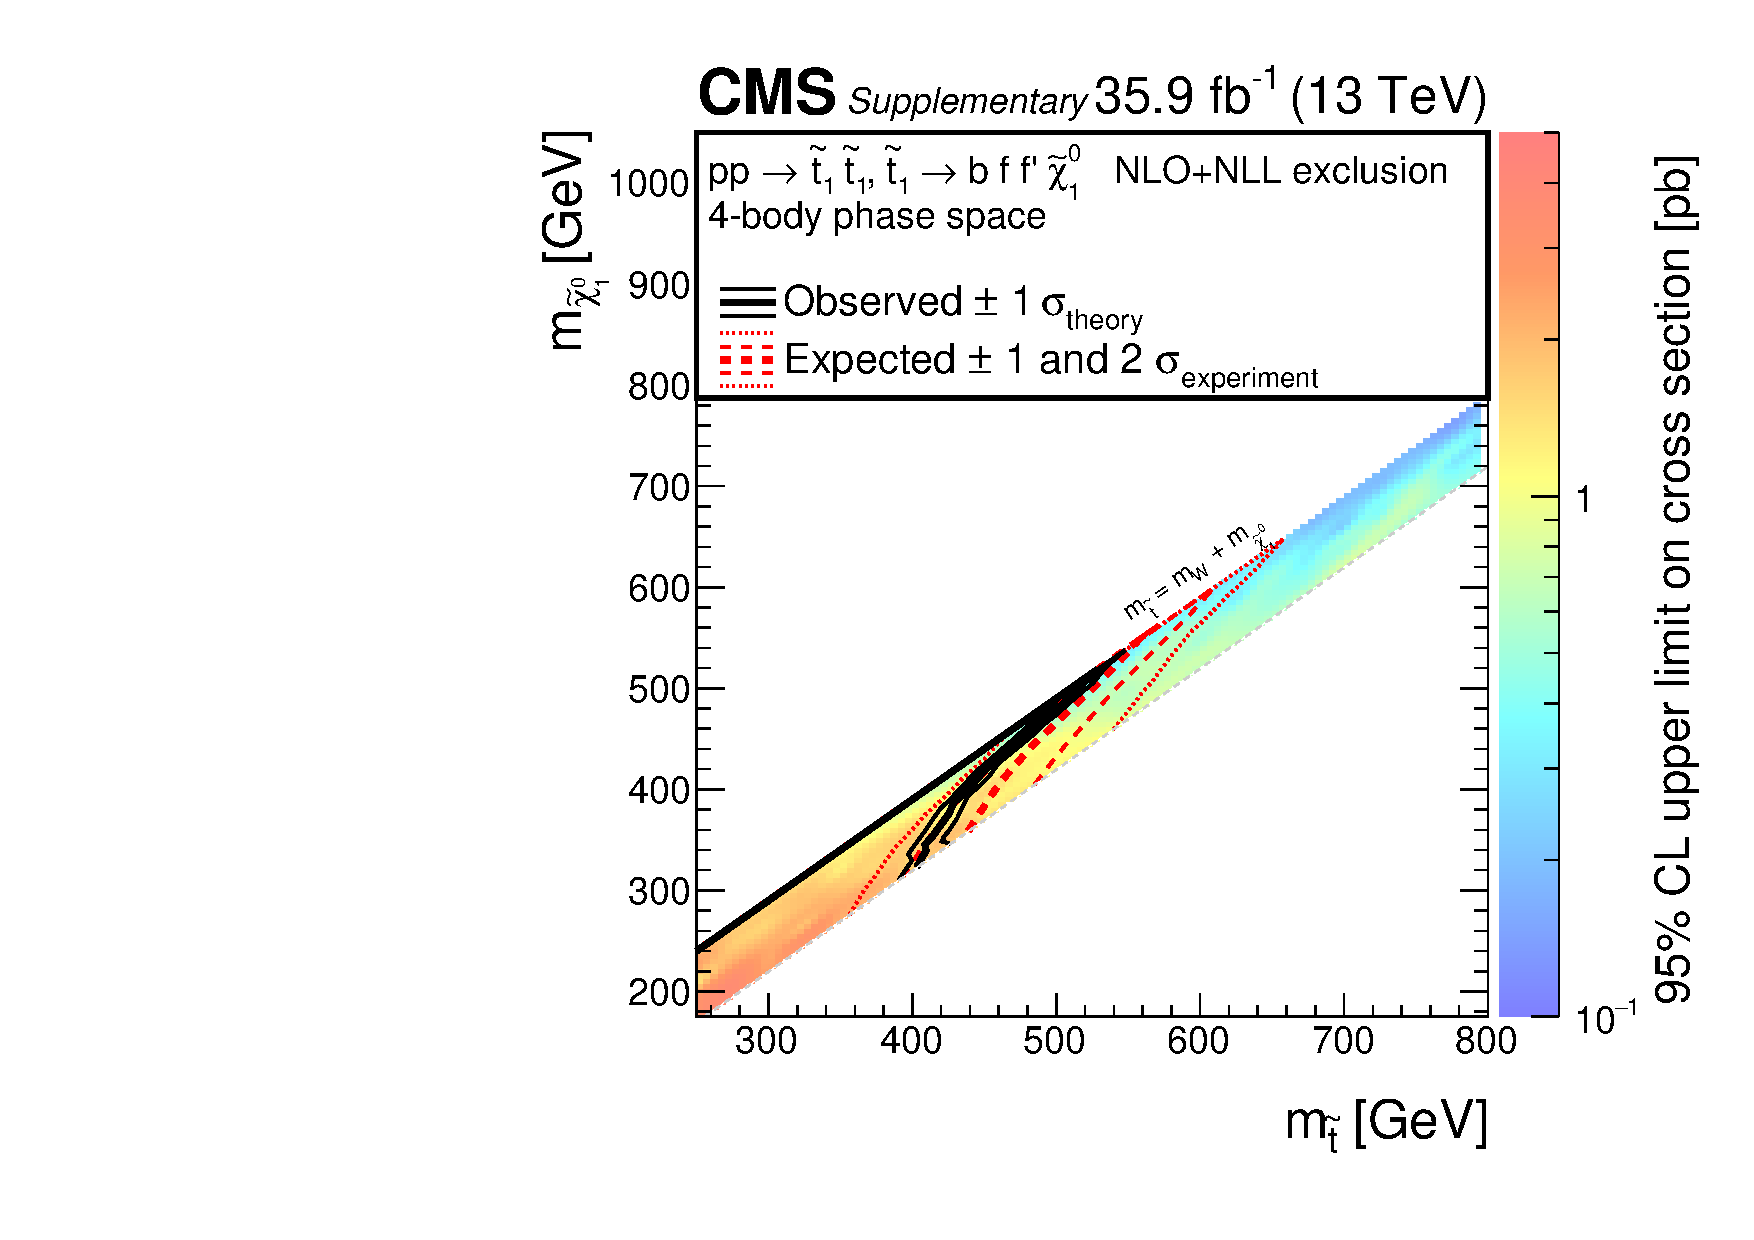
\includegraphics[width=120mm]{figures/T2-4bdXSEC.pdf}
\caption{T2tt-4bd: Upper limit on the cross section in the mass plane.}
\end{figure}

% UPDATE IF I MAKE CHANGES TO PLOT

Rob asked whether there was any signal contamination from the $\mu +$ jets CR, and it turns out there wasn't. This was a bug that appeared in some of the other SMS models as well, more evident in T1tttt and T2tt as they're more leptonic than the other models. The signal contamination should be most evident for mass splittings of $\sim 80\GeV$, as the sparticle can decay with an off-shell \PW boson that decays leptonically. The source of the bug was due to the trigger bit information not being in the trees (which I noticed previously when making the cut flow tables in Sec.~\ref{sec:cutflowtables2016paper}). However, we wouldn't need to regenerate the trees \emph{with} the trigger bits (as that would take ages), we'd just need to comment out \texttt{skimSequence.append(triggerSkimmer2016)} in \textbf{Sequences/Sequence2016.py} in AlphaTools. Then, I could just re-run the limits workflow from the StatsAnalyzer stage.


\subsection{Feynman diagram}

I could find the Feynman diagram at \url{https://twiki.cern.ch/twiki/pub/CMS/SUSYSimplifiedModelDiagrams/}. It is displayed below.

\begin{figure}[htbp]
\centering
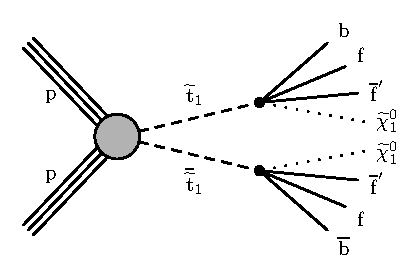
\includegraphics[width=80mm]{figures/T2tt-4bd_Feynman_diagram.pdf}
\caption{Graphical representation of the production and decay of supersymmetric particles in models with the production of third generation squarks (stops).}
\end{figure}


\subsection{Systematics for benchmarks}

For the systematic uncertainties, I can follow Shane's workflow at \url{https://github.com/shane-breeze/AlphaStats/wiki/Signal-systematic-studies}. Basically, I need to look at the systematics that are present in the AN and -- apart from MC stat. and luminosity -- see if they are in the list \texttt{runArguments.signalTemplatesFromFile} in \textbf{configStatFormula.py}. Then, I need to make sure those systematics are included in the \texttt{systList} list in \textbf{Scripts/makeSignalTemplateStudy.py}. I also need to make sure \texttt{"mcStat"} is in that list. Then, for AN-17-122, the list should look like

\begin{lstlisting}[belowskip=-0.7cm, language=python, numbers=none]
systList = [
    "nIsrWeight",
    "jecWeight",
    "puWeight",
    "bsfWeight",
    "bsfLightWeight",
    "bsfCFbWeight",
    "bsfCFlWeight",
    "bsfCFcWeight",
    "triggerWeight",
    "mcStat",
    ]
\end{lstlisting}

Then, I can run

\begin{lstlisting}[belowskip=-0.7cm, language=sh, numbers=none]
python Scripts/makeSignalTemplateStudy.py -i <datacard directory> -o <output directory> --filters <bechmark model>
\end{lstlisting}

A root file containing the systematic variations per njet, nb and HT bin is created in the output directory, and the systematic variations I need to include in the table in the AN are printed to the terminal. Note that the name of the systematic source isn't printed with each range, but they're printed in the order given in \texttt{sysList}. The luminosity uncertainty is usually just stated in the AN and is the same for each model, so I can just use that value. The strings \texttt{bsfCF+Weight} refer to the FastSim uncertainties. Replacing the "+" with a "b" is the b-tag uncertainty, "c" is for c-tags, and "l" is for light-tags. Then \texttt{bsfWeight} is the FullSim b-tag uncertainty and \texttt{bsfLightWeight} is the FullSim Mistag uncertainty.

\begin{landscape}
\begin{table}[htbp]
    \centering
    \small
    \begin{tabular}{ ccccccccccccc }
        \hline \hline
        Model & ($\mSusy,\mLSP$) & Luminosity & ISR & JEC & PU & b-tag & Mistag & b-tag & c-tag & light-tag & Trigger & MC stat. \\
        & & & & & & (Fullsim) & (Fullsim) & (Fastsim) & (Fastsim) & (Fastsim) & & \\ \hline
        T2tt-4bd & (450, 400) & 2.6\% & 4-20\% & 5-12\% & 7-12\% & 2-4\% & 2-3\% & 2-5\% & 2-5\% & 1-7\% & 2-3\% & 6-21\% \\
        \hline \hline
        \end{tabular}
    \caption{T2tt-4bd: Representative range taken from the $16\%$ and $84\%$ percentiles of the uncertainty across the analysis bins for each source of signal systematic. One benchmark point is chosen for this model, corresponding to the ``compressed'' scenario, i.e. with small mass splitting between the mother particle and the LSP.}
    \label{tab:T2tt-4bdSUS16038systs}
\end{table}
\end{landscape}

As a cross-check, I looked at the T2cc systematics as the values should be similar. They were, so I assume I've done everything correctly.

% MAKE THIS MORE CONVENIENT IF POSSIBLE


\subsection{Cross section limits for benchmarks}

The expected ($\mu_{\mathrm{exp}}$) and observed ($\mu_{\mathrm{obs}}$) upper limits on the production cross section are given in a table in the AN. For each of those limits, there are values for "nominal" and "simplified" binning. For nominal, the values should exist in the datacards I made when running the limits. Going into the datacard directory for the benchmark model, I need to look in the file \textbf{comb\_$<$model$>$\_mht\_card\_ASCLS\_UL\_PRIOR\_test.log\_$<$obs/exp$>$.txt} For the expected limit, there should be a line with \texttt{Expected 50.0\%: r < <number>}, where \texttt{<number>} is what I want. The value used for the cross section limit is always taken from the 50.0\% point. For the observed limit, there should be a line with \texttt{Observed Limit: r < <number>}.

For simplified, I need to re-run optimiseBinning, makeCardsAndWs and runCombineTask for the benchmark point (putting the output in a new directory for simplicity). But first, in \textbf{configStatFormula.py}, I need to set \texttt{doBenchmarks}  and \texttt{doSuperSignal} to \texttt{True}. These switch the binning from nominal to aggregated. I also had to add the benchmark mass points to \texttt{inputArguments.sigHists} under the \texttt{if doBenchMark:} statement. After the three steps have been run, I can follow the same procedure as nominal to get the simplified cross section limits.

\begin{table}[htbp]
  \centering
  \begin{tabular}{ llccccc }
    \hline
    \multicolumn{2}{c}{Benchmark models}    & \multicolumn{2}{c}{Nominal}
                                            &
                                            & \multicolumn{2}{c}{Simplified}             \\ [0.3ex]
    \cline{3-4}
    \cline{6-7}
    \multicolumn{2}{c}{$(m_{\text{SUSY}}, \mLSP)$ [GeV]}
                                            & $\mu_{\text{exp}}$
                                            & $\mu_{\text{obs}}$
                                            &
                                            & $\mu_{\text{exp}}$
                                            & $\mu_{\text{obs}}$                         \\ [0.3ex]
    \hline
    \texttt{T2tt-4bd} & (450, 400) & 0.94 & 1.89 & & 2.16 & 3.49 \\
        \hline
  \end{tabular}
  \caption{T2tt-4bd: Expected ($\mu_{\mathrm{exp}}$) and observed ($\mu_{\mathrm{obs}}$) upper limits on the production cross section, expressed in terms of the signal strength parameter, obtained using both the nominal and simplified binning schema.}
\end{table}

    
\subsection{Signal acceptance \texorpdfstring{$\times$}{x} efficiency}

This plot can be obtained in relatively few steps. I can run optimiseBinning in the same way as was used to calculate the limits, making sure the variables in \textbf{configStatFormula.py} were also the same (as I might have changed it when running other things). Then, I could run the following steps, referring to the output directory as \texttt{OUTDIR} as I did previously. I had to run makeCardsAndWs, combining \HT and $\nbjet$ with

\begin{lstlisting}[belowskip=-0.7cm, language=sh, numbers=none]
python makeCardsAndWs.py -i $OUTDIR -c "nB"
\end{lstlisting}

Then,

\begin{lstlisting}[belowskip=-0.7cm, language=sh, numbers=none]
python runCombineTask.py -i $OUTDIR -t ASCLS_UL_PRIOR --what expected
\end{lstlisting}

I could sort the \njet categories by sensitivity with

\begin{lstlisting}[belowskip=-0.7cm, language=sh, numbers=none]
python sortCategories.py -i $OUTDIR -m ul -c "nB"
\end{lstlisting}

Finally, I just had to add the StatsAnalyzer output directory (or StatsInput directory) to \texttt{inputFileStatsAnalyzer} in \textbf{makeJetRankingPlot\_2016\_SMS.py}, and could make the plots with

\begin{lstlisting}[belowskip=-0.7cm, language=sh, numbers=none]
python makeJetRankingPlot_2016_SMS.py -i $OUTDIR -o <output dir for plots>
\end{lstlisting}

This creates the plots of signal acceptance $\times$ efficiency for the mass plane, and also the plot of the most sensitive \njet categories. 

\begin{figure}[htbp]
\centering
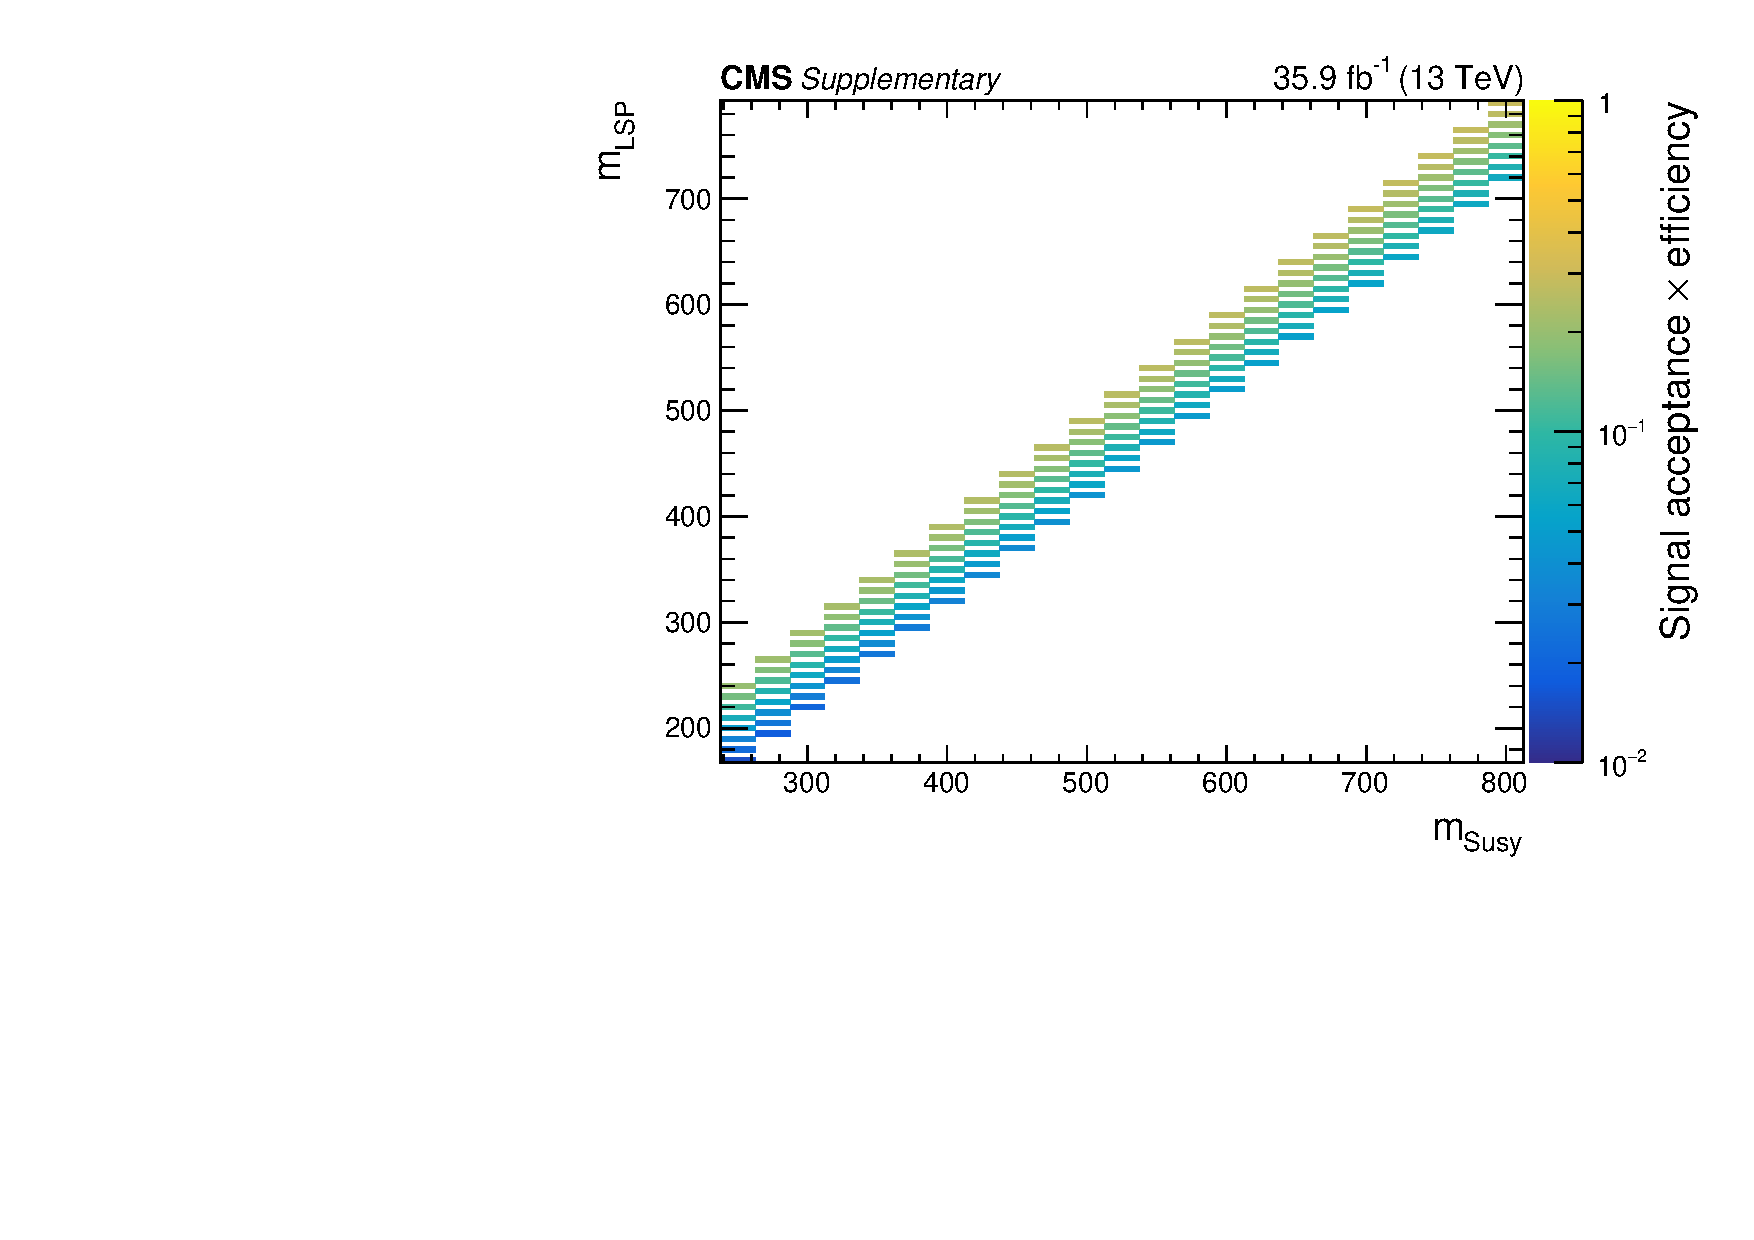
\includegraphics[width=120mm]{figures/T2tt_sig_acc_eff.pdf}
\caption{T2tt-4bd: $\epsilon_{\mathrm{sig}}$.}
\end{figure}

To extract the value for the benchmark model, need to go to the output directory, into the \textbf{eff/}. This should contain a root file with all the information in it. Then, in a \ROOT session, I can do

\begin{lstlisting}[belowskip=-0.7cm, language=C++, numbers=none]
TFile f("effHist.root")
f.ls() // To check the histograms
TH2D * h = (TH2D*)f.Get("T2tt_merging_7_cats")
h->GetBinContent(h->FindBin(450,400))
\end{lstlisting}

which gives me \textbf{0.0935877} for the benchmark model. In a nicer format:

\begin{table}[htbp]
    \caption{Signal efficiency for compressed T2tt-4bd model used in the analysis.}
    \label{tab:sig-effT2ttBenchmark}
    \centering
    \begin{tabular}{ ccc }
        \hline \hline
        Model & $(\mSusy,\mLSP)$ & Efficiency (total) \\
        \hline
        T2tt-4bd & (450, 400) & 9.4\% \\
        \hline \hline
        \end{tabular}
        \end{table}


\subsection{Most sensitive \texorpdfstring{\njet}{njet} categories}

This is accomplished when making the signal acceptance $\times$ efficiency plot. In the output directory from makeJetRankingPlot, there are separate plots for each \njet category, and the complete "bit map" plot. That is what needs to be added to the AN.

\begin{figure}[htbp]
\centering
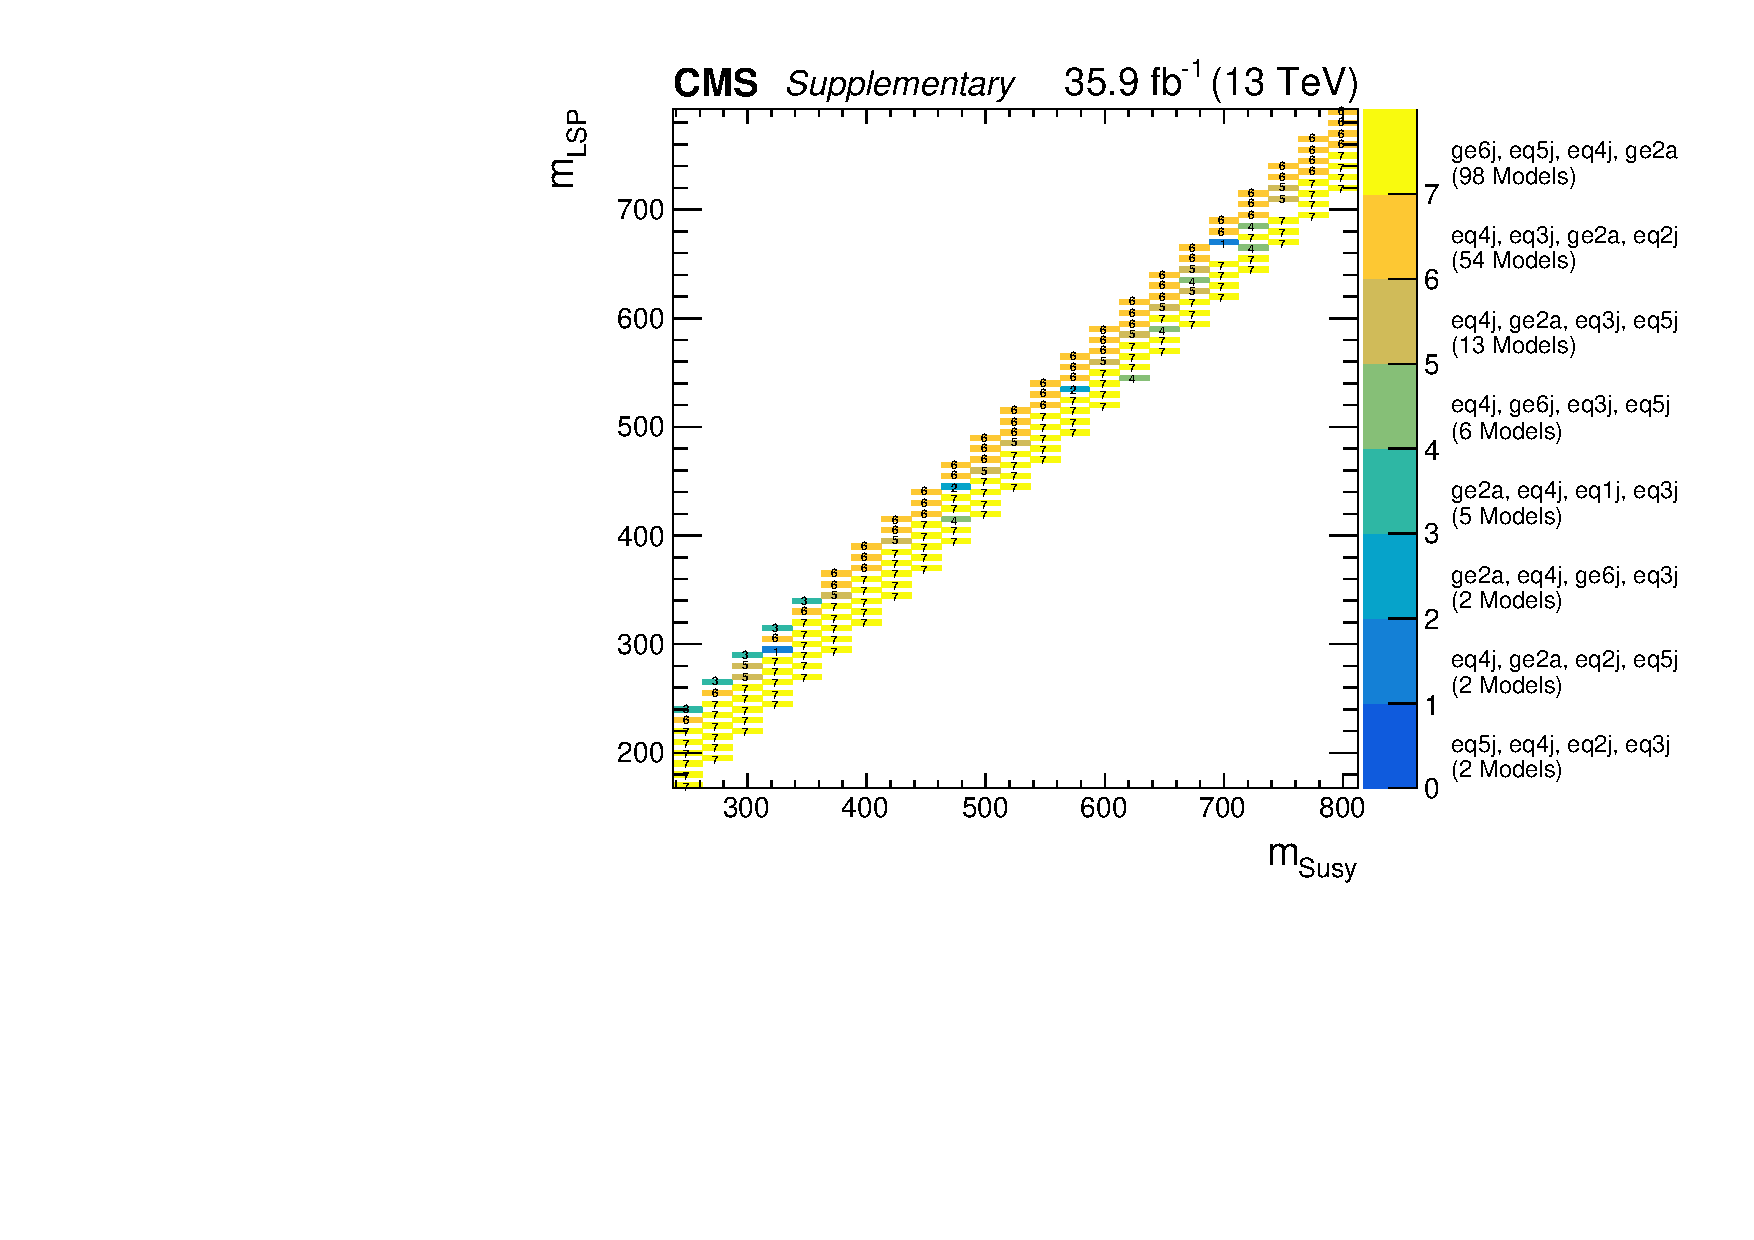
\includegraphics[width=120mm]{figures/T2tt_bitMap_improved.pdf}
\caption{T2tt-4bd: Most sensitive categories.}
\end{figure}


\subsection{Significance scan}

For the significance scan, I want to re-run optimiseBinning and makeCardsAndWs with the same arguments as when running limits, but in a new directory, which I'll label as \texttt{OUTDIR}. Then, I need to run runCombineTask with

\begin{lstlisting}[belowskip=-0.7cm, language=sh, numbers=none]
python runCombineTask.py -i $OUTDIR -t SIGNIF --what both
\end{lstlisting}

making sure \texttt{inputArguments.sigHists = "*"} in \textbf{configStatFormula.py} (as I might have changed it when running other things). In \textbf{PlotScripts/makeFinalPlane.py}, I had to comment out lines 272 (\texttt{wMassLine.Draw("same")}) and 274 (\texttt{tt.Draw("same")}) so the plot didn't show the dashed line with $\mSUSY - \mLSP = m_{\Ptop}$.  Finally, I can run

\begin{lstlisting}[belowskip=-0.7cm, language=sh, numbers=none]
python PlotScripts/makeFinalPlane.py --scenario observed --model "T2tt" -i $OUTDIR -o <output dir for plots> --mode pv --doubleTranspose --remake --remakePickle --smooth --task SIGNIF
\end{lstlisting}

to get the plots out. I want the interpolated version, which looks like this:

\begin{figure}[htbp]
\centering
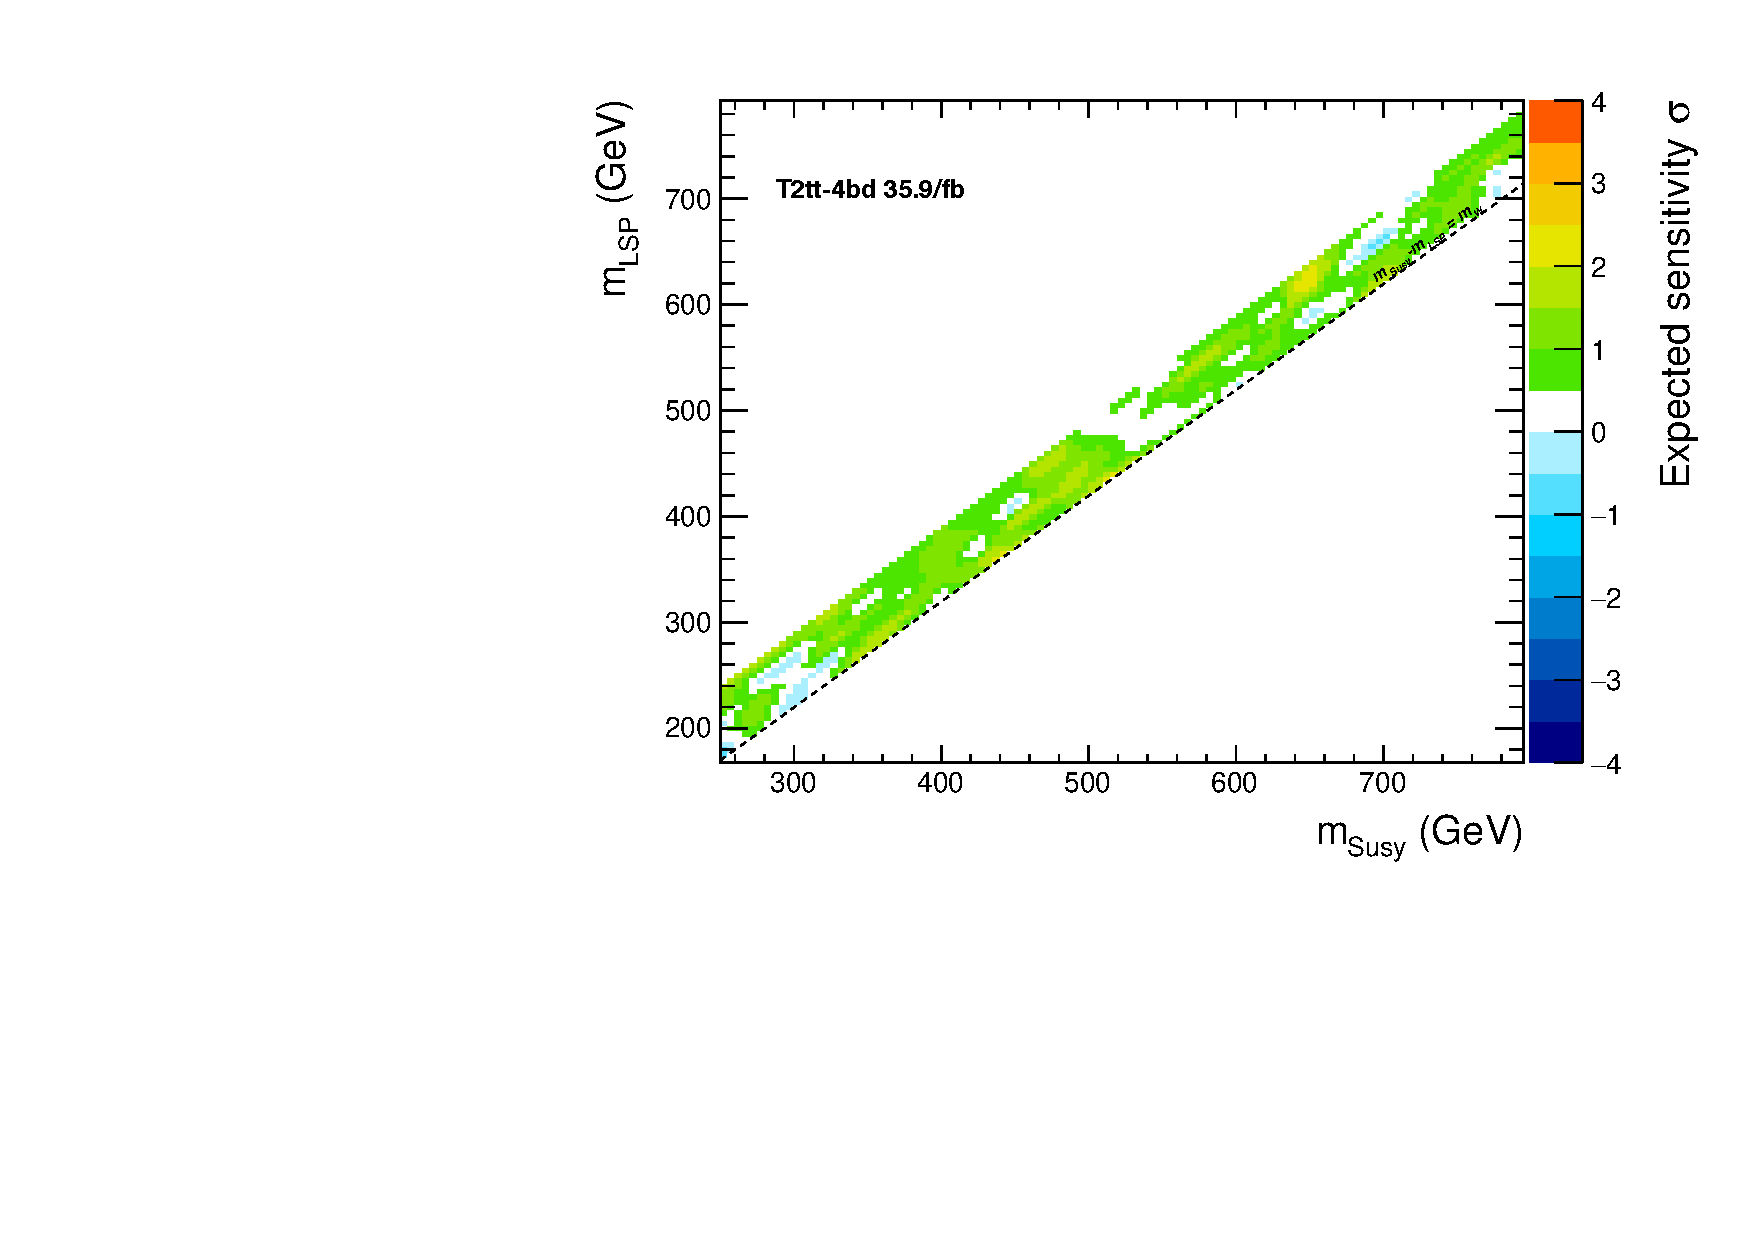
\includegraphics[width=110mm]{figures/Significance_scan.pdf}
\caption{T2tt-4bd: Significance scan.}
\end{figure}

I just had to change the text near the top left from "T2tt" to "T2tt-4bd".


\subsection{\texorpdfstring{$\sigma / \sigma_{\mathrm{theory}}$}{Sigma/sigma\_theory} (limits per bin) plots for benchmarks}

This is probably the most confusing part of the analysis. First, I had to edit \texttt{inputArguments.sigHists} in \textbf{configStatFormula.py} to include only the benchmark models (only one in this case). The rest of the environment should be set up as if I'm running limits (i.e., no \texttt{doSuperSignal}, etc.). Then, I had to run optimiseBinning on that model twice: once with the standard arguments when running limits; and once with the standard arguments plus the option \texttt{--gbForZinvExtrap}, which uses the greenband prediction for the $Z \rightarrow$ inv. $\nbjet$ extrapolation. The datacards generated must be in different directories, so I had to set the \texttt{-o} option to different paths. The commands would look like this:

\begin{lstlisting}[belowskip=-0.7cm, language=sh, numbers=none]
python batchSubmitOptimise.py -o <output dir without gb label> -f --options "--shapeSystFromFile --getDataLumi --runFormula --extrapolateZinv --greenBand" --submit
python batchSubmitOptimise.py -o <output dir with gb label> -f --options "--shapeSystFromFile --getDataLumi --runFormula --extrapolateZinv --greenBand --gbForZinvExtrap" --submit
\end{lstlisting}

Once done, I had to duplicate each of the output directories so I had four (two with \texttt{--gbForZinvExtrap} and two without). Then, I had to run makeCardsAndWs four times with different options for each. In one of the directories without \texttt{--gbForZinvExtrap}, I had to run with the option \texttt{-c "all"} to combine all bins, and in the other I had to run with \texttt{-c "nB"} to combine everything apart from \njet. Then, in one of the directories with \texttt{--gbForZinvExtrap}, I had to run with \texttt{-c "ht"} to combine only in \HT, and in the other directory I had to run with \texttt{-c "none"} to combine nothing. So, the commands would look like this:

\begin{lstlisting}[belowskip=-0.7cm, language=sh, numbers=none]
python makeCardsAndWs.py -i <datacards dir without gb 1> -c "all" --bbbFormulaUssr --bbbOptSig
python makeCardsAndWs.py -i <datacards dir without gb 2> -c "nB" --bbbFormulaUssr --bbbOptSig
python makeCardsAndWs.py -i <datacards dir with gb 1> -c "ht" --bbbFormulaUssr --bbbOptSig
python makeCardsAndWs.py -i <datacards dir with gb 2> -c "none" --bbbFormulaUssr --bbbOptSig
\end{lstlisting}

Once finished, I could run runCombineTask for each directory with the same arguments as limits:

\begin{lstlisting}[belowskip=-0.7cm, language=sh, numbers=none]
python runCombineTask.py -i <datacards dir> -t ASCLS_UL_PRIOR --what both
\end{lstlisting}

After that, I could go to the directory \textbf{dataframes/} and run

\begin{lstlisting}[belowskip=-0.7cm, language=sh, numbers=none]
python flatten_valid_bins.py -o ./flattened_bins.txt inputs/valid_bins.txt 
\end{lstlisting}

to make a flat list of the valid bins, using \textbf{inputs/valid\_bins.txt} as a template. Then, I went to \textbf{limitsPerBin/} to run \textbf{combineLimitsToDataframe.py} to create dataframes. Note that wildcarding is allowed, so I could specify the input directories like so:

\begin{lstlisting}[belowskip=-0.7cm, language=sh, numbers=none]
python combineLimitsToDataframe.py -i /vols/cms/RA1/80X/MC/20171026_T2tt_4bd/AlphaStats_Benchmark_* -o <output dir> --valid-bins ../flattened_bins.txt
\end{lstlisting}

X11 forwarding is required for the final step. So make sure to \texttt{ssh -Y}, then run \textbf{makeLimitPerBinPlots.py} with

\begin{lstlisting}[belowskip=-0.7cm, language=sh, numbers=none]
python makeLimitPerBinPlots.py -i <output dir from previous step> -o <output dir for plots>
\end{lstlisting}

which gives me the following plot for the benchmark model:

\begin{figure}[htbp]
\centering
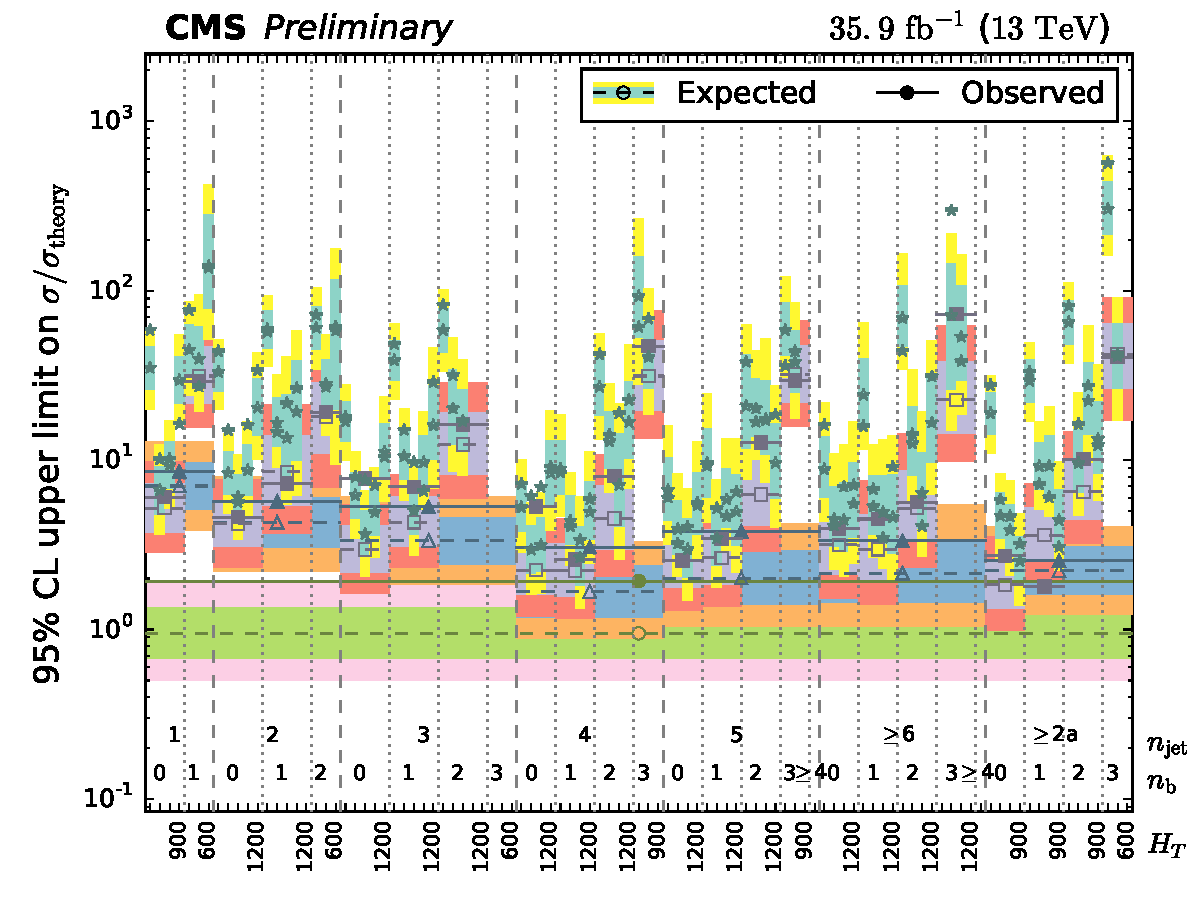
\includegraphics[width=120mm]{figures/SMS-T2tt_mStop-450_mLSP-400_25ns_limits_nj_nb_ht.pdf}
\caption{95\% CL upper limits on $\sigma / \sigma_{\mathrm{theory}}$ for the (450, 400) T2tt-4bd benchmark model are shown for four different bin combinations: no bins, \HT-only, ($\nbjet$, \HT) and all bins overlaid in ascending order. The expected limit, along with the $\pm 1 \sigma$ and $\pm 2 \sigma$ bands, and the observed limit are displayed for each bin.}
\end{figure}


\subsection{Mountain range plots for benchmarks}

Ben volunteered to make the mountain range plot for the benchmark model, as the README in AlphaStats was out of date. The plot is here:

\begin{figure}[htbp]
\centering
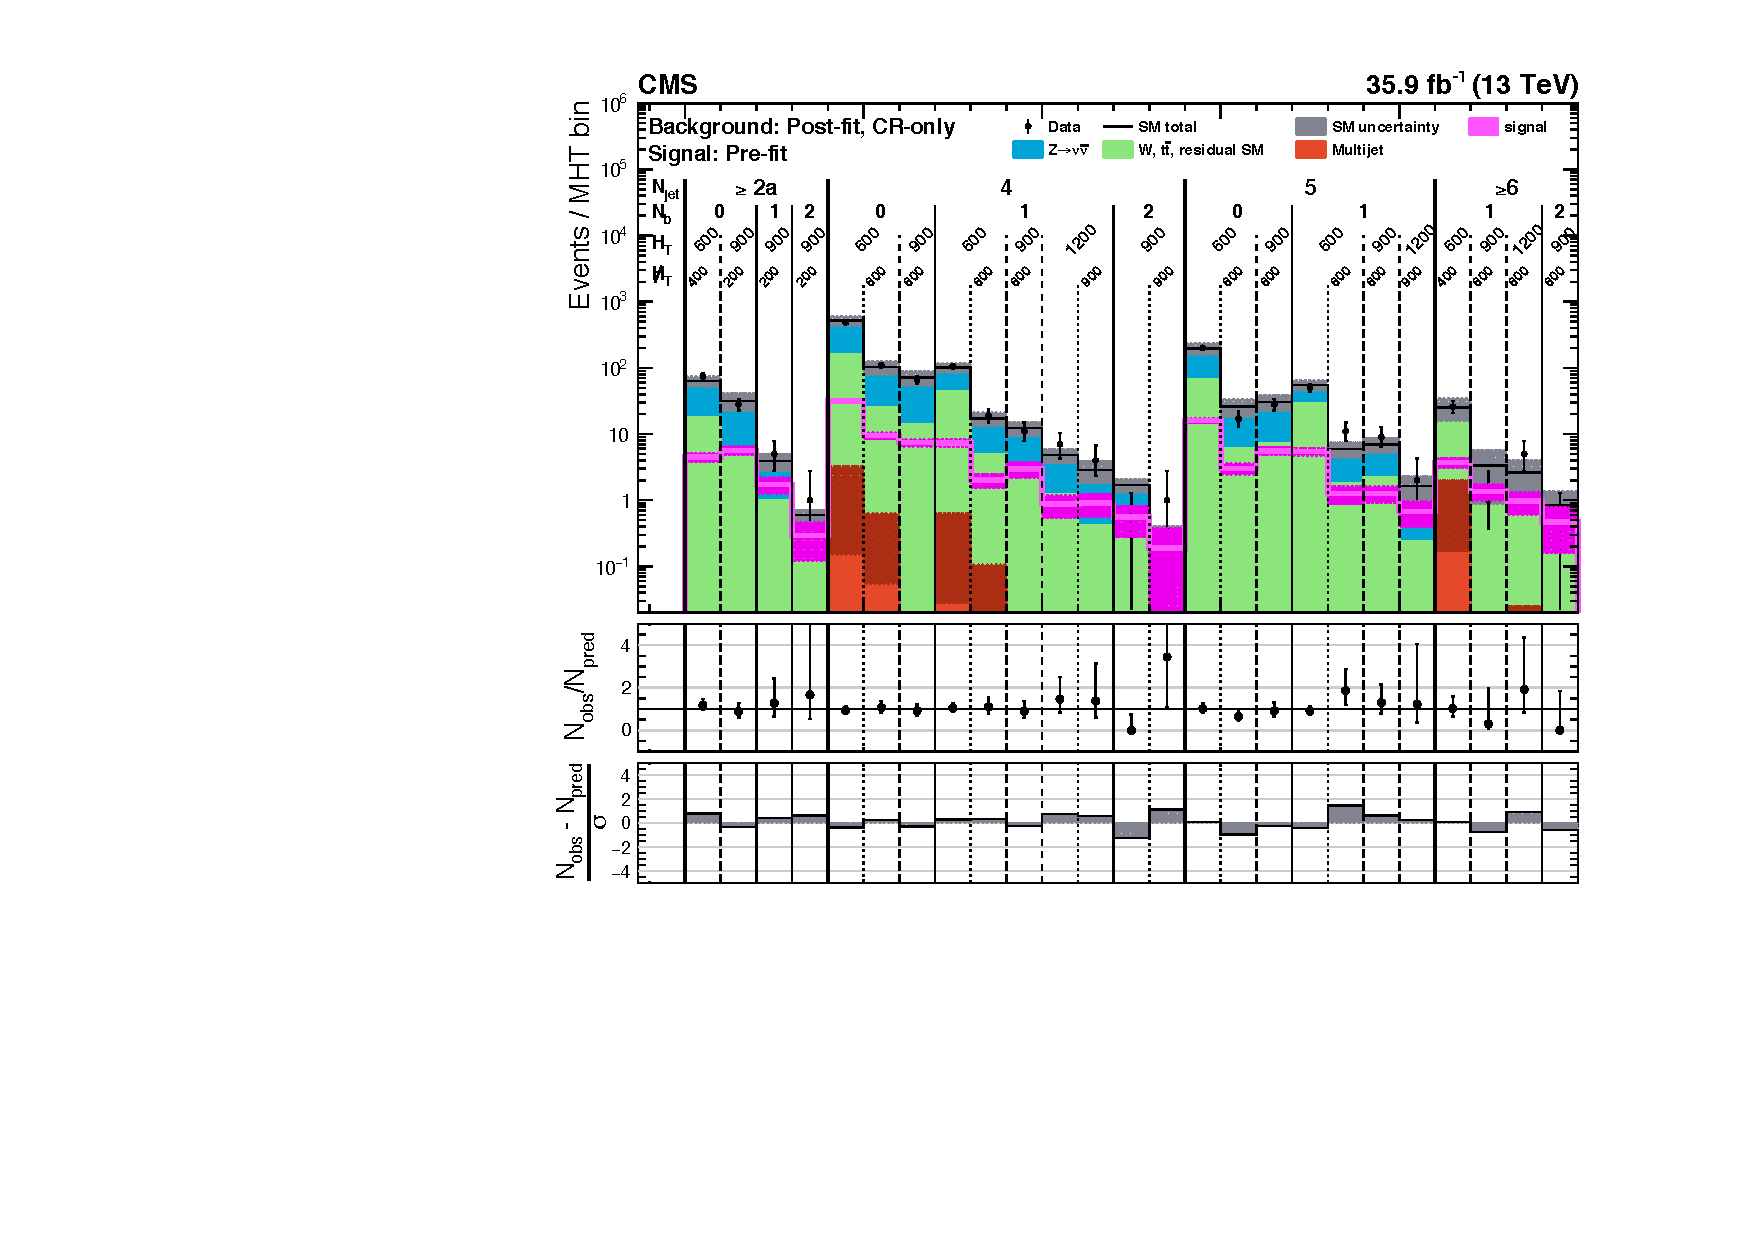
\includegraphics[width=140mm]{figures/all_full-fit-sig-top_bins_25.pdf}
\caption{Pre-fit T2tt-4bd benchmark model overlay on CR-only post-fit background prediction for the simplified bins. The uncertainty on the signal model counts represents the statistical uncertainty due to the finite size of the of the simulated sample.}
\end{figure}


\subsection{Cut flow table for benchmarks}

For the cut flows, I used the same workflow as in Section~\ref{sec:cutflowtables2016paper} to re-weight the split trees I already had for the benchmark model. I made sure to use the same branch of AlphaTools, just adding the sample to the T1qqqqLL sample file, and point to the ISR pickle I generated earlier for this model. Then, I could just point cutflowirl to the directory of the reweighted tree and run the code as normal to get the table.

\begin{table}[htbp]
\caption{Cut flow table for \texttt{T2tt-4bd} model.}
\resizebox{\textwidth}{!}{
\begin{tabular}{lc}
  \hline
  Event selection & \multicolumn{1}{c}{Benchmark model ($\mSUSY,\,\mLSP$)} \\
  \cline{2-2}
   & T2tt-4bd \\
    & (450,\,400) \\
  \hline
  Before selection  & 100\phantom{.1}  \\
  Event veto for muons and electrons & \phantom{1}79\phantom{.1} \\
  Event veto for single isolated tracks & \phantom{1}71\phantom{.1} \\
  Event veto for photons & \phantom{1}71\phantom{.1}  \\
  Event veto for jets failing ID & \phantom{1}71\phantom{.1}  \\
   $\njet \geq 2$  & \phantom{1}55\phantom{.1}  \\
   $0.1 <$ CHF$^{\jone} < 0.95$ & \phantom{1}50\phantom{.1}  \\
   $\ptjone > 100\GeV$ & \phantom{1}41\phantom{.1} \\
   $\HT > 200\GeV$  & \phantom{1}37\phantom{.1} \\
  $\mht > 200\GeV$  & \phantom{1}26\phantom{.1}  \\
  Event veto for forward jets ($\abseta > 2.4$) & \phantom{1}22\phantom{.1} \\
  $\mht / \etmiss < 1.25$ & \phantom{1}20\phantom{.1} \\
  \HT-dependent \alphat requirements ($\HT < 900\GeV$)  & \phantom{1}11\phantom{.1} \\
  $\biasedDPhi > 0.5$  & \phantom{10}8.3 \\
  \hline
\end{tabular}
}
\end{table}

% UPDATE CUT FLOW TABLE WITH CORRECT ONE


\section{Follow up and approval}

Once I added everything to the AN, I could build a draft copy to see how everything looked. If I went to \textbf{AlphaTDR2/}, I had to set up the environment with

\begin{lstlisting}[belowskip=-0.7cm, language=sh, numbers=none]
eval `notes/tdr runtime -sh`
\end{lstlisting}

Then I could build the pdf with

\begin{lstlisting}[belowskip=-0.7cm, language=sh, numbers=none]
cd notes/AN-17-122/trunk
tdr --draft --style=an b AN-17-122
\end{lstlisting}

Then the path to the pdf will be given.

I gave a presentation to RA1 about the analysis for this model: \href{run:modules/Sec 31 - Analysing the T2tt-4bd SUSY model/figures/T2tt-4bd analysis complete (16-11-2017).pdf}{T2tt-4bd analysis complete (16-11-2017)}. The main, interesting comments were about the limit per bin plot, the cut flow tables and the most sensitive \njet categories plot. Shane expected the $2b$ categories to drive the sensitivity in the limit per bin plot. But because the mass splitting is small, there's only a small amount of energy to be distributed among the \Pqb-jets, making them soft. With the cut flow tables, the same effect of the efficiencies not agreeing with the signal acceptance $\times$ efficiency values, applies here. The plot gives an efficiency of 9.4\%, while the table gives it as 8.3\%. I think this is due to the plot calculating the post-fit efficiency, while my tables calculate the pre-fit (because I only re-weight the trees). Then, in the \njet categories plot, two mass points were missing. In the raw plot, those two mass points were present but the values associated to their most sensitive categories were low, and so weren't included in the final plot. I don't think this is an issue as only 1\% of the models are affected.

I had to give an approval talk for the model at a SUSY inclusive meeting. The slides are here: \href{run:modules/Sec 31 - Analysing the T2tt-4bd SUSY model/figures/T20180213 T2tt-4bd approval.pdf}{20180213 T2tt-4bd approval}.


\section{Analysing the chargino-mediated model (T2bW\_X05, 03/04/2018)}

At the approval talk, one of the suggestions was to instead analyse the chargino-mediated model (sometimes referred to as "T2bW" or "T2bW\_X05") rather than the prompt decay model. Finding the Higgs at 125 GeV gives this model a better chance of being found over the prompt decay. In this version, the stop decays into a chargino and \Pqb, with the chargino decaying into the LSP and \PW: $p \rightarrow \tilde{t} \bar{\tilde{t}}, \ \tilde{t} \rightarrow b\tilde{\chi}^{\pm}, \ \tilde{\chi}^{\pm} \rightarrow W^* \tilde{\chi}_1^0$.

I used CMSSW\_8\_0\_25 with my fork of \emph{cmgtools-lite-private}, the CMGTools branch \emph{80X-ra1-0.7.x-Moriond17Prod-EshSUSYcutflow2016} and added the dataset \textbf{/SMS-T2bW\_\-X05\_\-dM-10to80\_\-genHT-160\_\-genMET-80\_\-mWMin-0p1\_\-TuneCUETP8M1\_\-13TeV-madgraphMLM-pythia8/RunIISpring16MiniAODv2-PUSpring16Fast\_\-80X\_\-mcRun2\_\-asymptotic\_\-2016\_\-miniAODv2\_\-v0-v1/MINIAODSIM} to the components. I ran AtLogicNoSelection to make the flat trees, storing them at \textbf{/vols/cms/RA1/80X/MC/20180329\_\-S01/} on Imperial and analysed them in virtually the same fashion as the prompt model.

When I split the trees, I had to rename the directories to "SMS-T2bW\_\-X05\_\-$<$blah$>$" and make sure the model name "T2bW\_\-X05" was uncommented in the various files in AlphaTools I needed to use. I then had to \emph{manually} make a sample file containing all the directory names because of how the splitting works and the troublesome underscore in the model name. I could import that file in the scripts \textbf{samples\_\-13TeV\_\-80X.py} (where I also had to add the line \texttt{sampleList80X.addSampleHandler("<collection name>")}) and \textbf{Analyzers/StatsInput/produceShellScript.py}. Then, I could add the name of the collection to \texttt{psetSignalModels2016.sampleSelection} in \textbf{Analyzers/NIsrAnalyzer/NIsrAnalyzer\_cfg.py} and run the script to get the ISR weights in a root file. I then had to change the signal model in \textbf{compileSignalNormPickle.py} and run that to get the pickle file. Once completed, I had to add the model and collection name to \texttt{sampleListDict} in \textbf{produceShellScript.py} and could then run the StatsAnalyzer steps as normal. The subsequent AlphaStats steps were also the same, bearing in mind the model name.

The plots and tables for the analysis are below.

\begin{figure}[htbp]
\centering
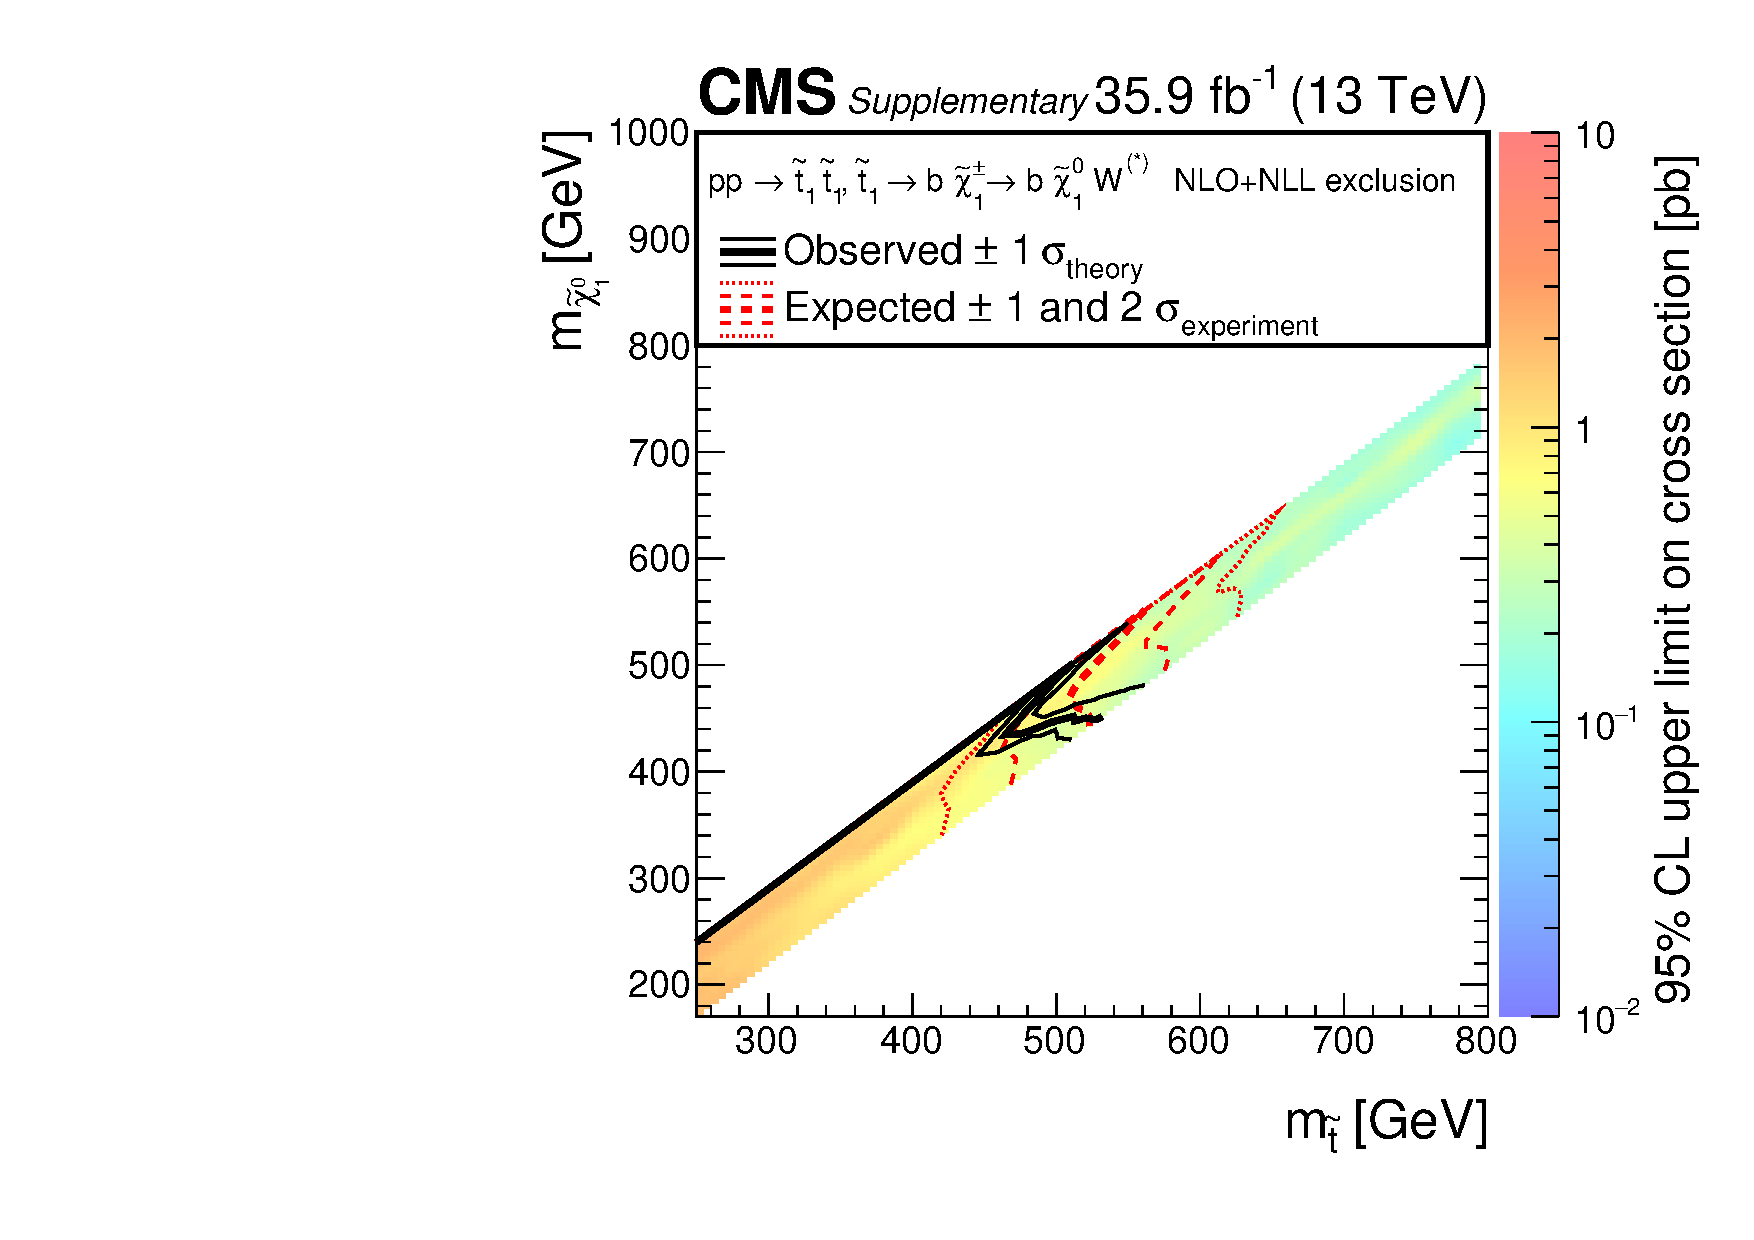
\includegraphics[width=120mm]{figures/T2bW/T2bW_X05XSEC.pdf}
\caption{T2bW\_X05: Upper limit on the cross section in the mass plane.}
\end{figure}

% REMEMBER TO UPDATE IF CHANGES NEED TO BE MADE (E.G. CROSS SECTION)

\begin{figure}[htbp]
\centering
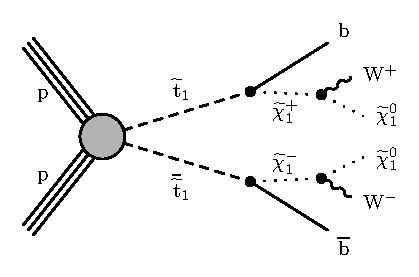
\includegraphics[width=80mm]{figures/T2bW/T2bW_Feynman.pdf}
\caption{Graphical representation of the production and decay of supersymmetric particles in models with the production of third generation squarks (stops).}
\end{figure}

We chose a benchmark model at (500, 460). Usually, when choosing benchmark points, we want to choose a point near the expected exclusion. From the limit plot, (500, 460) seemed like the best option. Below is the table of systematic uncertainties for the benchmark model.

\begin{landscape}
\begin{table}[htbp]
    \centering
    \small
    \begin{tabular}{ ccccccccccccc }
        \hline \hline
        Model & ($\mSusy,\mLSP$) & Luminosity & ISR & JEC & PU & b-tag & Mistag & b-tag & c-tag & light-tag & Trigger & MC stat. \\
        & & & & & & (Fullsim) & (Fullsim) & (Fastsim) & (Fastsim) & (Fastsim) & & \\ \hline
        T2bW\_X05 & (500, 460) & 2.6\% & 4-22\% & 4-13\% & 8-12\% & 2-4\% & 1-2\% & 2-5\% & 3-7\% & 1-8\% & 2-2\% & 7-21\% \\
        \hline \hline
        \end{tabular}
    \caption{T2bW\_X05: Representative range taken from the $16\%$ and $84\%$ percentiles of the uncertainty across the analysis bins for each source of signal systematic. One benchmark point is chosen for this model, corresponding to the ``compressed'' scenario, i.e. with small mass splitting between the mother particle and the LSP.}
    \label{tab:T2bWSUS16038systs}
\end{table}
\end{landscape}

\begin{table}[htbp]
  \centering
  \begin{tabular}{ llccccc }
    \hline
    \multicolumn{2}{c}{Benchmark models}    & \multicolumn{2}{c}{Nominal}
                                            &
                                            & \multicolumn{2}{c}{Simplified}             \\ [0.3ex]
    \cline{3-4}
    \cline{6-7}
    \multicolumn{2}{c}{$(m_{\text{SUSY}}, \mLSP)$ [GeV]}
                                            & $\mu_{\text{exp}}$
                                            & $\mu_{\text{obs}}$
                                            &
                                            & $\mu_{\text{exp}}$
                                            & $\mu_{\text{obs}}$                         \\ [0.3ex]
    \hline
    \texttt{T2bW\_X05} & (500, 460) & 0.9961 & 1.8094 & & 2.1953 & 3.4695 \\
        \hline
  \end{tabular}
  \caption{T2bW\_X05: Expected ($\mu_{\mathrm{exp}}$) and observed ($\mu_{\mathrm{obs}}$) upper limits on the production cross section, expressed in terms of the signal strength parameter, obtained using both the nominal and simplified binning schema.}
\end{table}

\iffalse
\begin{figure}[htbp]
\centering
\includegraphics[width=120mm]{figures/???}
\caption{T2bW\_X05: $\epsilon_{\mathrm{sig}}$.}
\end{figure}

\begin{figure}[htbp]
\centering
\includegraphics[width=120mm]{figures/???}
\caption{T2bW\_X05: Most sensitive categories.}
\end{figure}
\fi

\begin{figure}[htbp]
\centering
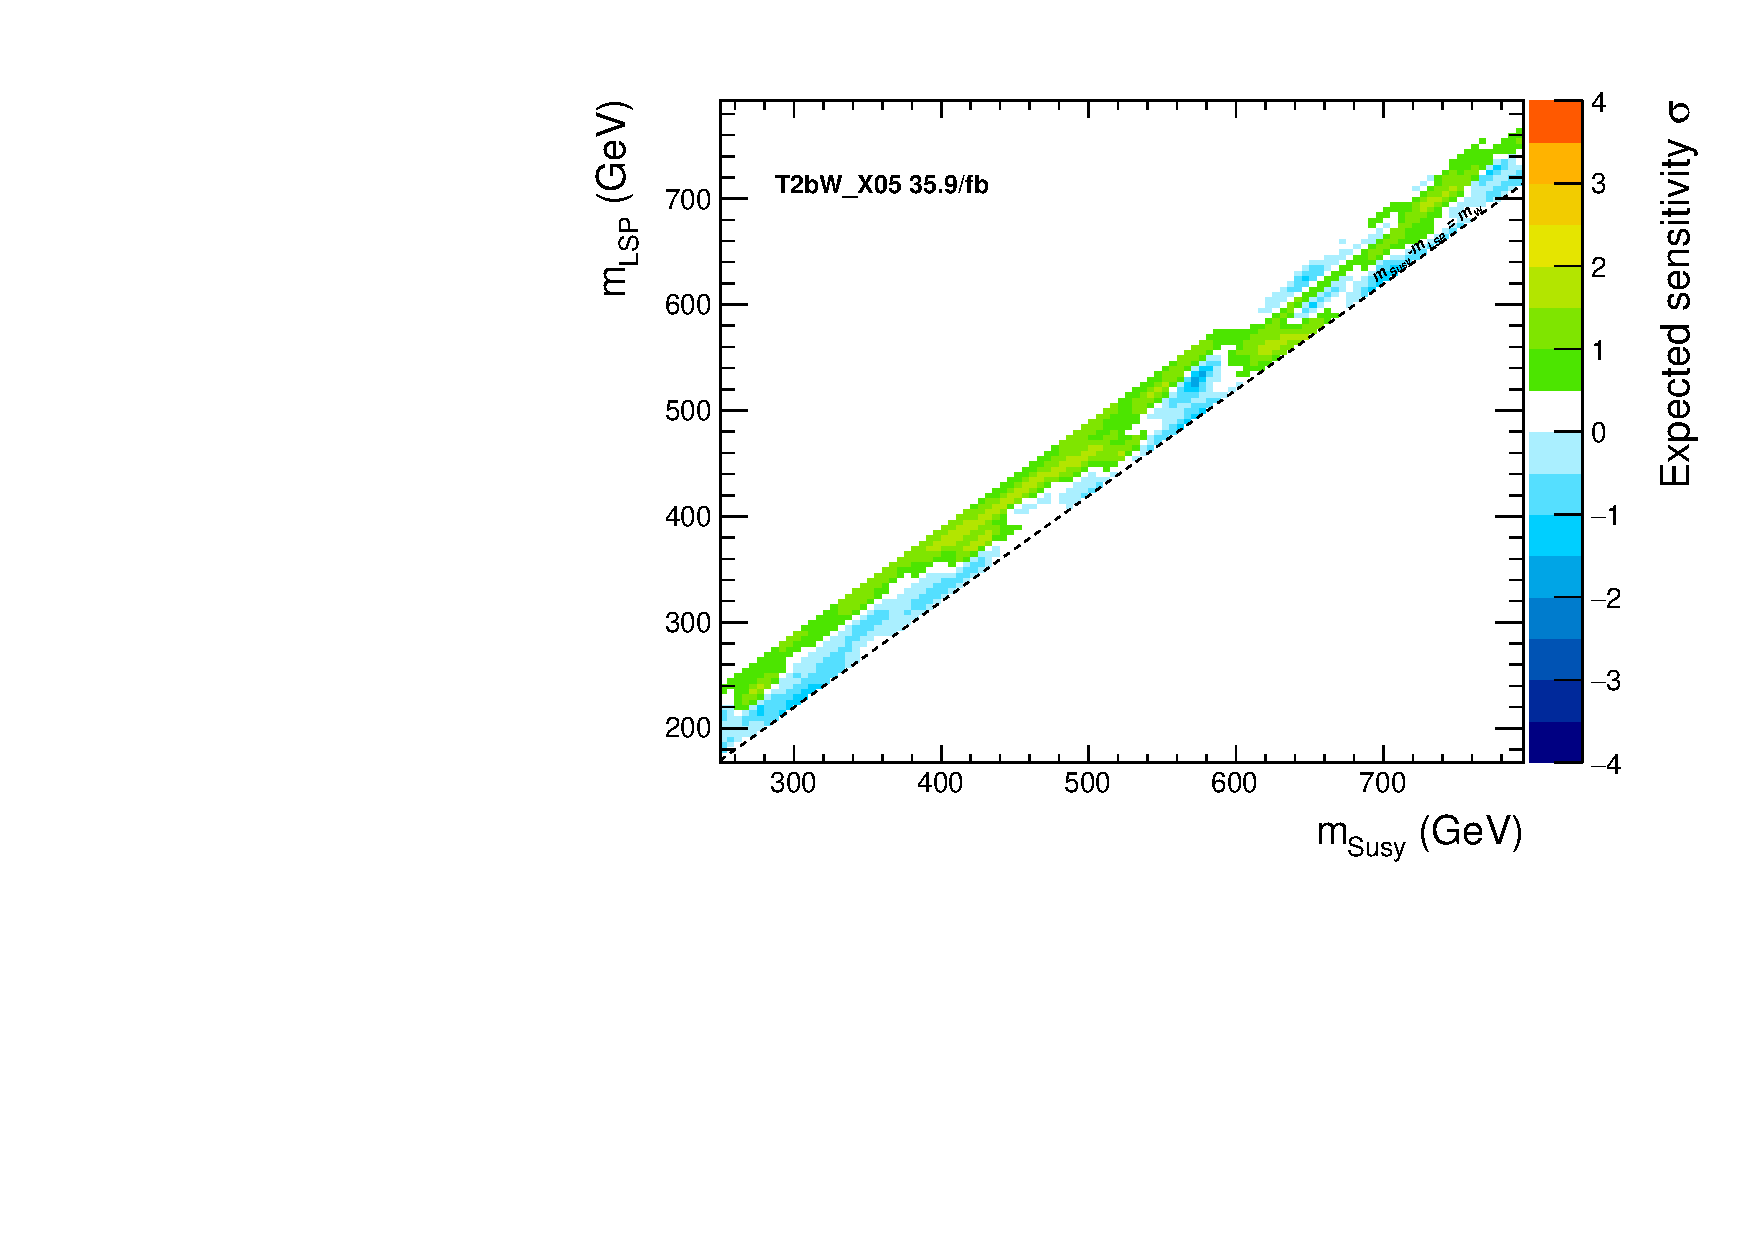
\includegraphics[width=110mm]{figures/T2bW/finalCanvasObsSignif.pdf}
\caption{T2bW\_X05: Significance scan.}
\end{figure}

\begin{figure}[htbp]
\centering
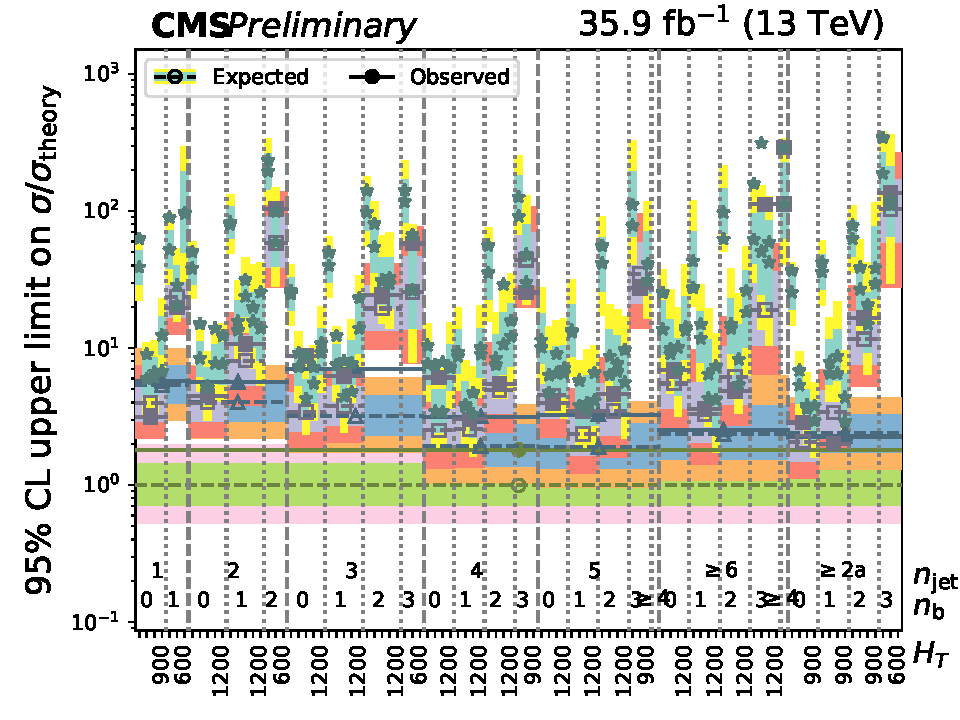
\includegraphics[width=120mm]{figures/T2bW/SMS-T2bW_X05_mStop-500_mLSP-460_25ns_limits_nj_nb_ht.pdf}
\caption{95\% CL upper limits on $\sigma / \sigma_{\mathrm{theory}}$ for the (500, 460) T2bW\_X05 benchmark model are shown for four different bin combinations: no bins, \HT-only, ($\nbjet$, \HT) and all bins overlaid in ascending order. The expected limit, along with the $\pm 1 \sigma$ and $\pm 2 \sigma$ bands, and the observed limit are displayed for each bin.}
\end{figure}


% NEED TO ADD Signal acceptance $\times$ efficiency for benchmark model, Plot of the most sensitive \njet categories, Mountain range plots for benchmark model, Cut flow tables for benchmark model (ask Ben)

% Fix cross section reweighting for both models. Would need to remake limit plane (find out where xs is applied and just multiply it by the factor), signal acc x eff (again, just multiply xs by the factor, ~L152 in makeJetRankingPlot_2016), limit per bin plots.
